%! Author = Luca
%! Date = 18.12.2022

Für die erfolgreiche Entwicklung der geplanten Datenbank sind eine sorgfältige Ressourcenplanung, ein detaillierter Zeitplan und eine realistische Budgetplanung erforderlich.
Die folgende Ressourcenplanung, Zeitplan und Budget sollen dazu beitragen, das Projekt erfolgreich zu planen und durchzuführen.

\subsection{Ressourcenplan}
\begin{itemize}
    \item Projektleiter: 1 Person (50\% Zeitaufwand)
    \item Softwareentwickler: 2 Personen (100\% Zeitaufwand)
    \item Projektassistent: 1 Person (50\% Zeitaufwand)
    \item Qualitätssicherung: 1 Person (50\% Zeitaufwand)
\end{itemize}

\subsection{Zeitplan}
\begin{itemize}
    \item Phase 1: Anforderungsanalyse und Konzeption (2 Wochen)
    \item Phase 2: Entwicklung (6 Wochen)
    \item Phase 3: Test und Qualitätssicherung (2 Wochen)
    \item Phase 4: Implementierung und Dokumentation (1 Woche)
\end{itemize}

\subsection{Budget}
\begin{itemize}
    \item Personalkosten: 50.000 €
    \item Lizenzen und Werkzeuge: 10.000 €
    \item Reisekosten: 2.000 €
    \item Sonstige Kosten: 5.000 €
\end{itemize}
Gesamtbudget: 67.000 €

\subsection{Erstellung des Datenbank Models}
Die Erstellung eines ERM-Modells (Entity Relationship Model) ist ein wichtiger Bestandteil der Projektplanung bei der Erstellung einer Datenbank.
Das ERM-Modell dient dazu, die Struktur der Daten in der Datenbank zu beschreiben und die Beziehungen zwischen verschiedenen Entitäten (also Objekten oder Konzepten) darzustellen.\\

Das in \figref{fig:erm} dargestellte ERM-Modell zeigt die Beziehungen zwischen verschiedenen Entitäten (also Objekten oder Konzepten) in der geplanten Datenbank für die Schäfer \& Twachtmann Immobilien GbR.

\begin{figure}[H]
    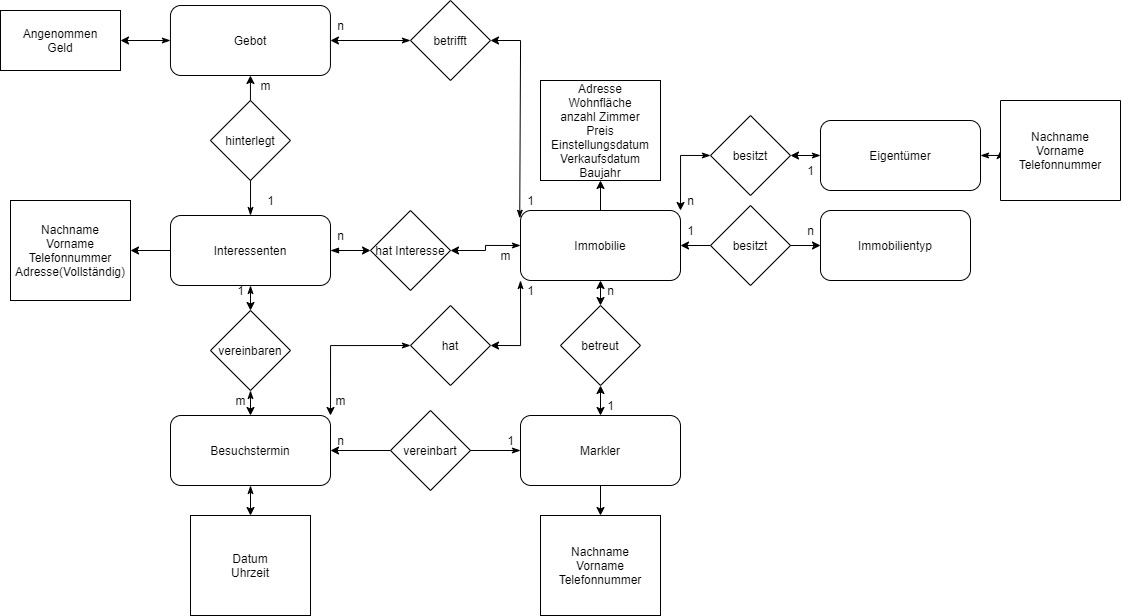
\includegraphics[width=\textwidth]{images/Immobilien_ERD}
    \caption{ERM-Model}
    \label{fig:erm}
\end{figure}

Die Entität ``Immobilie'' wird durch die Attribute ``Adresse'', ``Wohnfläche'', ``Anzahl der Zimmer'', ``Preis'', ``Einstellungsdatum'', ``Verkaufsdatum'' und ``Baujahr'' beschrieben.
Es gibt auch eine Beziehung zur Entität ``Immobilientyp'', die verschiedene Typen von Immobilien wie Einfamilienhäuser, Mehrfamilienhäuser, Reihenmittelhäuser und Reihenendhäuser umfasst.
Jede Immobilie wird von einem Makler betreut, wobei jeder Makler über einen uneindeutigen Nachnamen, Vornamen und eine Telefonnummer verfügt.
Die Eigentümer jeder Immobilie werden ebenfalls mit Vornamen, Nachnamen und Telefonnummer gespeichert.\\

Das Maklerbüro hat auch Stammkunden, die im Laufe der Jahre immer wieder Immobilien über das Maklerbüro angeboten haben.
Als Interessenten bezeichnet das Büro Leute, die die Immobilien kaufen wollen.
Sie werden mit Nach- und Vornamen, vollständiger Adresse und Telefonnummer erfasst.
Mit Interessenten vereinbart der Makler an einem bestimmten Datum zu einer bestimmten Uhrzeit Besuchstermine.
Wenn der Interessent an einer Immobilie interessiert ist, hinterlegt er ein Gebot.
In der Datenbank wird gespeichert, ob das Gebot angenommen wurde oder nicht.\\

Das ERM-Modell zeigt auch, dass es zwischen den Entitäten ``Interessent'' und ``Gebot'' sowie zwischen ``Makler'' und ``Besuchstermin'' eine 1:n-Beziehung gibt.
Das bedeutet, dass ein Interessent mehrere Gebote abgeben und ein Makler mehrere Besuchstermine vereinbaren kann, aber umgekehrt gibt es nur ein Interessenten-Gebot pro Gebot und nur einen Makler pro Besuchstermin.\\

Das ERM-Modell gibt somit einen Überblick über die Struktur und Beziehungen der Daten in der geplanten Datenbank für die Schäfer \& Twachtmann Immobilien GbR und dient als Basis für die weitere Planung und Entwicklung der Datenbank.
